\documentclass[%
reprint,
russian,
%superscriptaddress,
%groupedaddress,
%unsortedaddress,
%runinaddress,
%frontmatterverbose, 
%preprint,
%preprintnumbers,
%nofootinbib,
%nobibnotes,
%bibnotes,
 amsmath,amssymb,
 aps,
%pra,
%prb,
%rmp,
%prstab,
%prstper,
%floatfix,
]{revtex4-2}

\usepackage{cases}
\usepackage[T2A]{fontenc}
\usepackage[russian]{babel}   %% загружает пакет многоязыковой вёрстки
\usepackage{graphicx}% Include figure files
\usepackage{dcolumn}% Align table columns on decimal point
\usepackage{bm}% bold math
\usepackage{hyperref}% add hypertext capabilities
\usepackage{xcolor}
%\usepackage[mathlines]{lineno}% Enable numbering of text and display math
%\linenumbers\relax % Commence numbering lines

\definecolor{linkcolor}{HTML}{0000D5} % цвет ссылок
\definecolor{urlcolor}{HTML}{0000D5} % цвет гиперссылок
 
\hypersetup{pdfstartview=FitH,  linkcolor=linkcolor,urlcolor=urlcolor, colorlinks=true}
 
%\usepackage[showframe,%Uncomment any one of the following lines to test 
%%scale=0.7, marginratio={1:1, 2:3}, ignoreall,% default settings
%%text={7in,10in},centering,
%%margin=1.5in,
%%total={6.5in,8.75in}, top=1.2in, left=0.9in, includefoot,
%%height=10in,a5paper,hmargin={3cm,0.8in},
%]{geometry}

\usepackage{etoolbox}
\makeatletter
% \frontmatter@RRAP@format is responsible for the parentheses
\patchcmd{\frontmatter@RRAP@format}{(}{}{}{}
\patchcmd{\frontmatter@RRAP@format}{)}{}{}{}
\renewcommand\Dated@name{}
\makeatother

\begin{document}


%\preprint{APS/123-QED}

\title{Лабораторная работа 3:\\Интерферометр Майкельсона}% Force line breaks with \\
%\thanks{A footnote to the article title}

\author{Никитин Илья}
 \altaffiliation[]{Факультет физики, НИУ ВШЭ}%Lines break automatically or can be forced with \\
 \email{isnikitin_1@edu.hse.ru}
% It is always \today, today,
             %  but any date may be explicitly specified
 \date{27 мая 2021г.}
\begin{abstract}
В данной лабораторной изучены принципы работы интерферометра Майкельсона, найдены коэффициенты преломления нескольких пластинок из орг-стекла, найдена спектральная ширина лазера и сделаны оценки теплового коэффициента расширения стали.
\end{abstract}

\maketitle

\tableofcontents

\section{\label{sec:level1}Конструкция установки и теория}

В первой части мы рассмотрим базовую конструкцию интерферометра Майкельсона и проведем некоторые теоретические выкладки, которые послужат основой для проводимых экспериментов

\subsection{\label{sec:level2}Конструкция}

\begin{figure}[h!]
\includegraphics[width=1\linewidth]{Scheme.png}% Here is how to import EPS art
\caption{\label{fig:epsart} Схема установки. 1 -- лазер; 2 -- делительный куб; 3,4 -- зеркала; 5 -- экран}
\end{figure}
Луч лазера (1), попадая на делительный куб (2), делится на отраженный и прошедший лучи, далее отражаясь от зеркал (3) и (4) соответственно и снова попадая на делительный куб, откуда попадают на экран (5), образуя интерференционную картину.

\subsection{\label{sec:level2}Теория}
\subsubsection{\label{sec:level3}Интерференционные максимумы и минимумы}
Интенсивность света, полученная при интерференции от двух источников, излучающих плоские монохроматические волны с разностью фаз $\Delta \phi$:
\begin{equation*}
    \begin{split}
   		\begin{aligned}
   			I \sim \langle \mathbf{E}^2_1 \cos(\mathbf{kr} - \omega t)|^2 \rangle_t +
   			\langle |\mathbf{E}^2_2 \cos(\mathbf{kr} - \omega t + \delta \phi)|^2 \rangle_t\\
   			+ \langle |\mathbf{E}_1 \mathbf{E}_2\cos(\mathbf{kr} - \omega t)\cos(\mathbf{kr} - \omega t + \delta \phi)| \rangle_t
   		\end{aligned}
   	\end{split}
\end{equation*}
Применяя формулу косинуса суммы и предполагая интенсивности источников равными, получим:
\begin{equation}
    \label{Intensity}
    I = 2 I_0 (1 + \cos{\delta\mathbf{\phi}})
\end{equation}
Исходя из полученного соотношения, зная, что $\delta \phi = \frac{2 \pi}{\lambda} \Delta$, где $\Delta$ - разность хода, а $\lambda$ -- длина волны, получаем условие максимумов и минимумов интерференционной картины:
\begin{numcases}{\Delta =}
    m \lambda \text{ -- условие максимума}  \label{maximum}
    \\
    (m + 1/2) \lambda \text{ -- условие минимума} \label{minimum}
\end{numcases}
\subsubsection{\label{sec:level3}Получение длины волны источника}
Нетрудно понять, что двигая одно из зеркал на длину $\delta x$, разность хода составит $2\delta x$, отсюда, с использованием уравнения \ref{maximum}, получим следующее соотношение:
\begin{equation}
    \label{wavelength}
    2 \delta x = N \lambda
\end{equation}
где $N$ -- количество переходов максимум/минимум
\subsubsection{\label{sec:level3}Интерферометр как спектральный прибор}
Получим аналог формулы \ref{Intensity} для случая, когда источники имеют разные длины волн.
\begin{equation*}
    \begin{split}
   		\begin{aligned}
   			I \sim \langle \mathbf{E}^2_1 \cos(\mathbf{k_1 r} - \omega t)|^2 \rangle_t +
   			\langle |\mathbf{E}^2_2 \cos(\mathbf{k_2 r} - \omega t + \delta \phi)|^2 \rangle_t\\
   			+ \langle |\mathbf{E}_1 \mathbf{E}_2\cos(\mathbf{k_1r} - \omega t)\cos(\mathbf{k_2 r} - \omega t + \delta \phi)| \rangle_t
   		\end{aligned}
   	\end{split}
\end{equation*}
Перепишем полученную формулу в более удобном виде:
\begin{equation*}
    \begin{split}
   		\begin{aligned}
        	I \sim (1 + 1 + \cos[k_1 \Delta] + \cos[k_2 \Delta]) = (2 \\
        	+ \cos[(k_1 + k_2) \Delta / 2]) (\cos[(k_1 - k_2)\Delta/2])
   		\end{aligned}
   	\end{split}
\end{equation*}
Откуда получается условие минимума контрастности:
\begin{equation*}
    (\frac{\pi}{\lambda_1} - \frac{\pi}{\lambda_2}) \Delta = \pi (m + 1/2)
\end{equation*}
Предполагая длины волн достаточно близкими, можно переписать это выражение следующим образом:
\begin{equation}
    \label{Spectrum}
    \Delta = (m + 1/2) \frac{\lambda_0^2}{2\Delta \lambda}
\end{equation}
\subsubsection{\label{sec:level3}Определение показателя преломления с помощью интерферометра}
Если перед зеркалом поставить пластинку из орг стекла, то с помощью описанной установки можно определить показатель преломления.
\begin{figure}[h!]
\includegraphics[width=1\linewidth]{Scheme2.png}% Here is how to import EPS art
\caption{\label{fig:epsart}Схематичное изображение пластинки в двух различных положениях}
\end{figure}
Пусть $D_1$ и $D_2$ -- оптические пути для пластинки, соответственно, перпендикулярной падающему свету и находящейся под углом $\alpha$ к лучу.
\begin{equation*}
    \begin{cases}
        D_1 = L1 + L2 + nt\\
        D_2 = L1 + L2 + nw - \Delta L1 + \Delta L2
    \end{cases}
\end{equation*}
Отсюда получаем разность хода:
\begin{equation}
    \label{eq1}
    \Delta = n(w - t) - \Delta L1 + \Delta L2 = N \lambda
\end{equation}
Выразим все неизвестные величины через ширину пластинки $t$ и углы:
\begin{equation}
    \label{eq2}
    \begin{cases}
        \Delta L1 = t \tan{\beta} \sin{\alpha}\\
        \Delta L2 = t (1 + \cos{\alpha}(\frac{\tan{\beta}}{\tan{\alpha}} - 1))\\
        w = \frac{t}{cos{\beta}}
    \end{cases}
\end{equation}
Воспользуемся законом Снелла:
\begin{equation}
    \label{eq3}
    \sin{\alpha} = n \sin{\beta} \Rightarrow \cos{\beta} = \sqrt{1 - \frac{\sin^2{\alpha}}{n^2}}
\end{equation}
Наконец, пользуясь соотношениями \ref{eq1}, \ref{eq2}, \ref{eq3}, получим:
\begin{equation}
    N \lambda = 2 t (\sqrt{n^2 - \sin^2{\alpha}} + 1 - \cos{\alpha} - n)
\end{equation}
Перепишем соотношение в удобном для нас виде, выразив коэффициент преломления:
\begin{equation}
    \label{refraction}
    n = \frac{(\frac{N \lambda}{2t} + \cos{\alpha} - 1)^2 + \sin^2{\alpha}}{2 (-\frac{N \lambda}{2t} - \cos{\alpha} + 1)}
\end{equation}
\subsubsection{\label{sec:level3}Коэффициент теплового расширения}
Воспользуемся основным законом теплового приближения:
\begin{equation*}
    L = L_0 \exp[\alpha \Delta T]
\end{equation*}
В той постановке эксперимента, которая будет описана в дальшейшем можно использовать линейное приближение данного закона:
\begin{equation*}
    \Delta L = L_0 \alpha \Delta T
\end{equation*}
Воспользуемся уравнением \ref{wavelength} и заключим:
\begin{equation}
    \label{heat}
    N = \frac{\alpha \Delta T L_0}{\lambda}
\end{equation}
\section{Ход работы}
\subsection{Изменение длины плеча}
\subsubsection{Результат эксперимента}
В результате эксперимента наблюдалось изменение интерференционной картины в зависимости от длины плеча. С изменением расстояния до зеркала, максимумы сменяли минимумы и наоборот.
\subsubsection{Размышление над результатами}
Согласно уравнению \ref{Intensity}, интенсивность зависит от разности фаз, которая линейно зависит от разности хода. Таким образом, меняя длину плеча, можно наблюдать на экране изменение интерференционной картины.
\subsection{Поднесение спички к падающему лучу}
\subsubsection{Результат эксперимента}
В результате эксперимента наблюдалось изменение интерференционной картины при поднесении спички. Максимумы сменяли минимумы и наоборот.
\subsubsection{Размышление над результатами}
Рассуждения аналогичны предыдущим, отличие заключается в причине изменения разности хода. Там менялось плечо, здесь же меняется коэффициент преломления из-за изменения температуры воздуха.
\subsection{Наблюдение второй интерференционной картины}
Очевидно, что используемая система часть света пропускает в сторону лазера. Если поставить делительную пластину между кубом и лазером, то выйдет пронаблюдать две картины на одном экране.
\subsubsection{Результат эксперимента}
В результате эксперимента получилось следующее изображение на экране:
\begin{figure}[h!]
\includegraphics[width=1\linewidth]{Interferention.png}
\caption{\label{fig:epsart}Интерференционные картины, полученные на экране}
\end{figure}
\subsubsection{Размышление над результатами}
Примечательно, что на одной части экрана наблюдается деструктивное изображение, а на другой конструктивное. Такое наблюдение можно объяснить законом сохранения энергии.
\subsection{Измерение длины волны излучения}
С помощью интерферометра можно получить длину волны лазера. Используем для этого формулу \ref{wavelength}. Меняя смещение плеча интерферометра, будем считать количество переходов максимум/минимум, а затем расчитаем длину волны. 
\subsubsection{Результат эксперимента}
В ходе эксперимента получились следующие результаты:
\begin{table}[h!]%The best place to locate the table environment is directly after its first reference in text
\begin{ruledtabular}
\begin{tabular}{lcdr}
\textrm{Сдвиг зеркала, мкм}&
\textrm{Количество переходов}\\
\colrule
12 & 43\\
17 & 60\\
22 & 79\\
14 & 50\\
13 & 46\\
\end{tabular}
\end{ruledtabular}
\end{table}
\subsubsection{Обработка данных}
По полученым данным построим график:
\begin{figure}[h!]
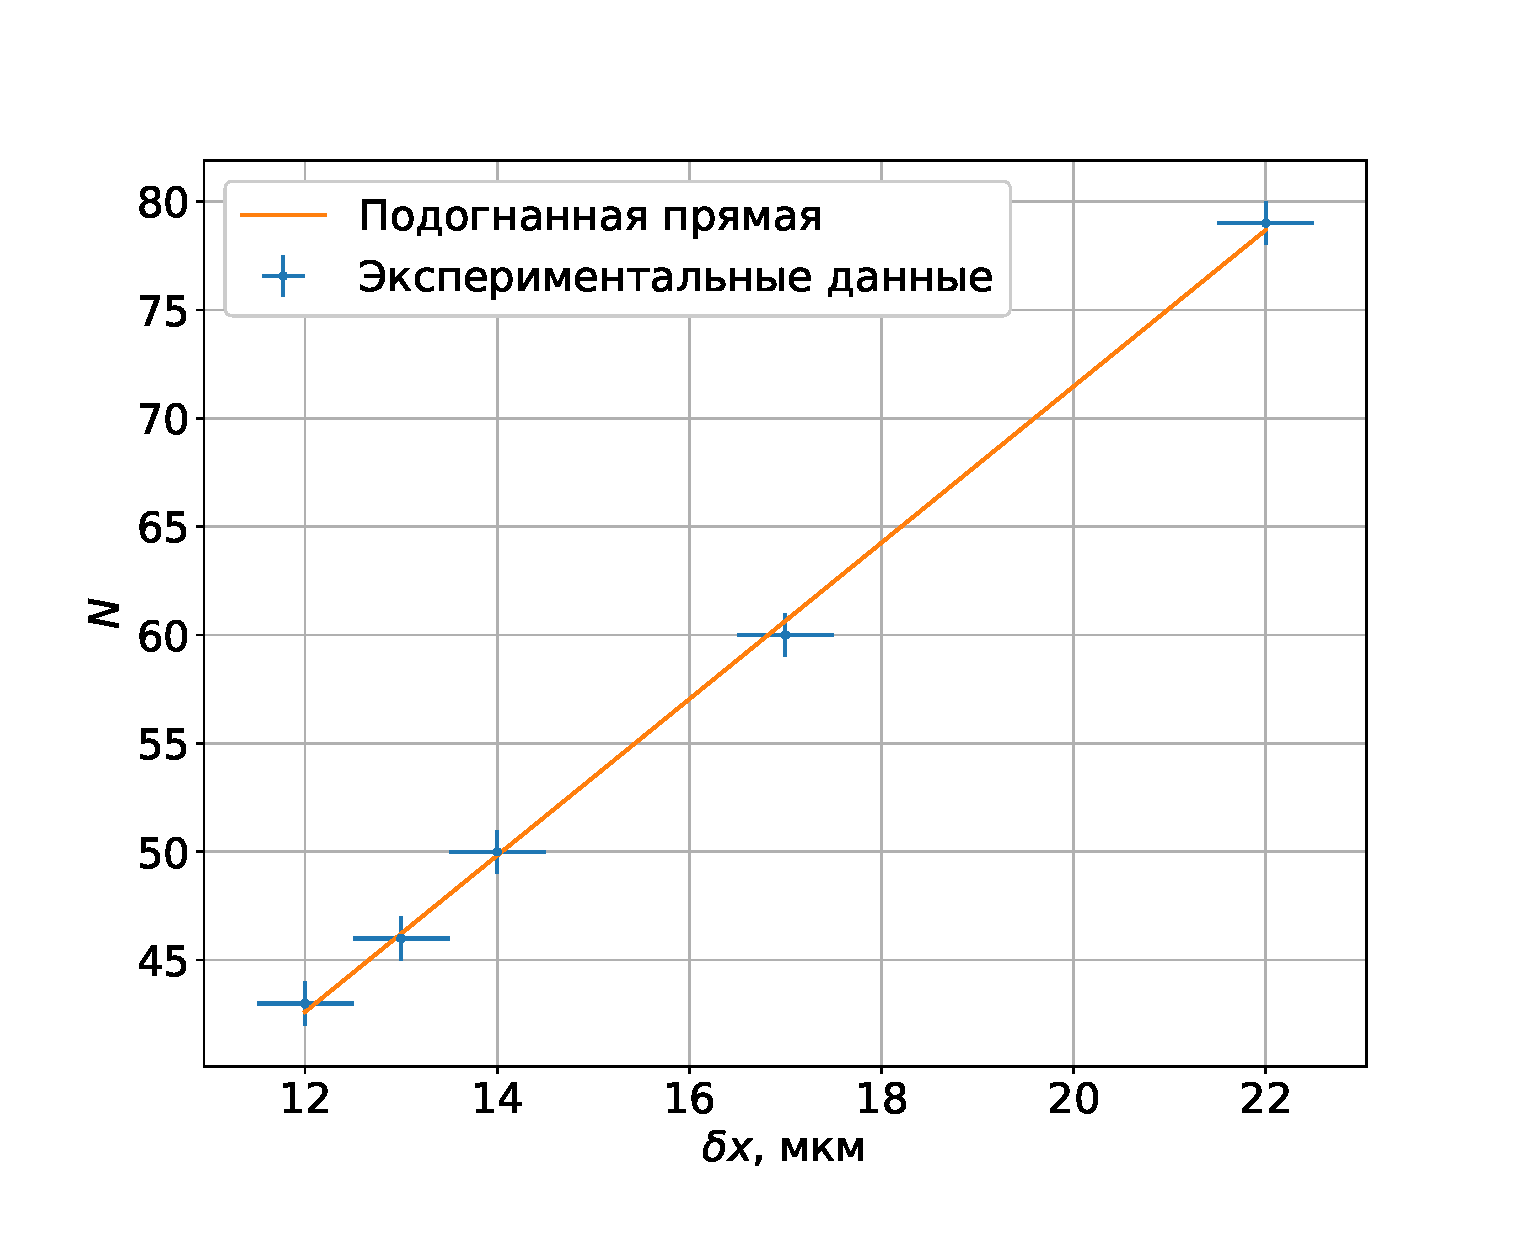
\includegraphics[width=1\linewidth]{exp3.eps}
\caption{\label{fig:epsart}График зависимости количества переходов от сдвига зеркала}
\end{figure}
В результате подгонки прямой, получили некоторое значение коэффициента ее наклона, который с легкостью можно пересчитать в длину волны: $\lambda = 554 \pm 38$ нм
\subsection{Измерение ширины спектра}
Интерферометр можно использовать как спектральный прибор. Для этого необходимо найти такое положение зеркала, при котором будет наблюдаться минимальный контраст. Исходя из результатов, полученных в соотношении \ref{Spectrum}, расстояние между положениями минимального контраста выражается через ширину спектра.
\subsubsection{Результат эксперимента}
После того, как был найден минимальный контраст, нами был произведен поиск следующего положения минимального контраста. Это положение находилось на расстоянии $\approx 975$ мкм, что соответствует ширине спектра $\Delta \lambda \approx 0.15$ нм.
\subsection{Измерение показателя преломления стеклянной пластинки}
С помощью интерферометра можно определить показатель преломления стеклянной пластинки. Воспользуемся результатом теоретических выкладок, а конкретно формулой \ref{refraction}. Согласно формуле, для определения коэффициента преломления, достаточно знать толщину пластинки, угол ее отклонения и число переходов между максимумами и минимумами интерференционной картины.
\subsubsection{Результаты эксперимента}
В ходе эксперимента получились следующие результаты:
\begin{table}[h!]
\caption{Измерения с тонкой пластинкой}
\begin{ruledtabular}
\begin{tabular}{lcdr}
\textrm{Количество переходов}&
\textrm{Угол, минут}\\
\colrule
5 & 95\\
10 & 145\\
15 & 185\\
20 & 215\\
25 & 240\\
30 & 265\\
40 & 300
\end{tabular}
\end{ruledtabular}
\end{table}
\begin{table}[h!]
\caption{Измерения с толстой пластинкой}
\begin{ruledtabular}
\begin{tabular}{lcdr}
\textrm{Количество переходов}&
\textrm{Угол, минут}\\
\colrule
10 & 120\\
25 & 215\\
30 & 225\\
35 & 230\\
40 & 265\\
50 & 300\\
60 & 330
\end{tabular}
\end{ruledtabular}
\end{table}
\subsubsection{Обработка данных}
По полученым данным вычислим коэффициенты преломления:
\begin{equation}
    \begin{cases}
        n_{\text{тонкая}} = 1.59 \pm 0.03 \\
        n_{\text{толстая}} = 1.43 \pm 0.05\\
    \end{cases}
\end{equation}
\subsection{Измерение коэффициента теплового расширения}
Прикрепим на зеркало стальной прутик, по которому будем пускать ток. Прутик начнет нагреваться, удлинняться и двигать зеркало, которое в свою очередь будет изменять интерференционную картину по закону, описанному формулой \ref{heat}. Температуру будем измерять обычной термопарой на мультиметре, а переходы интерференционной картины, вместе с показаниями мультиметра будем записывать на видео.
\subsubsection{Результат эксперимента}
\begin{table}[h!]
\begin{ruledtabular}
\begin{tabular}{lcdr}
\textrm{Температура, $C^\circ$}&
\textrm{Количество переходов}\\
\colrule
23 & 0\\
24 & 3\\
25 & 8\\
26 & 17\\
27 & 25\\
28 & 33\\
29 & 40\\
30 & 47\\
31 & 54\\
32 & 61\\
33 & 68\\
34 & 76\\
39 & 98\\
\end{tabular}
\end{ruledtabular}
\end{table}
\subsubsection{Обработка данных}
\begin{figure*}
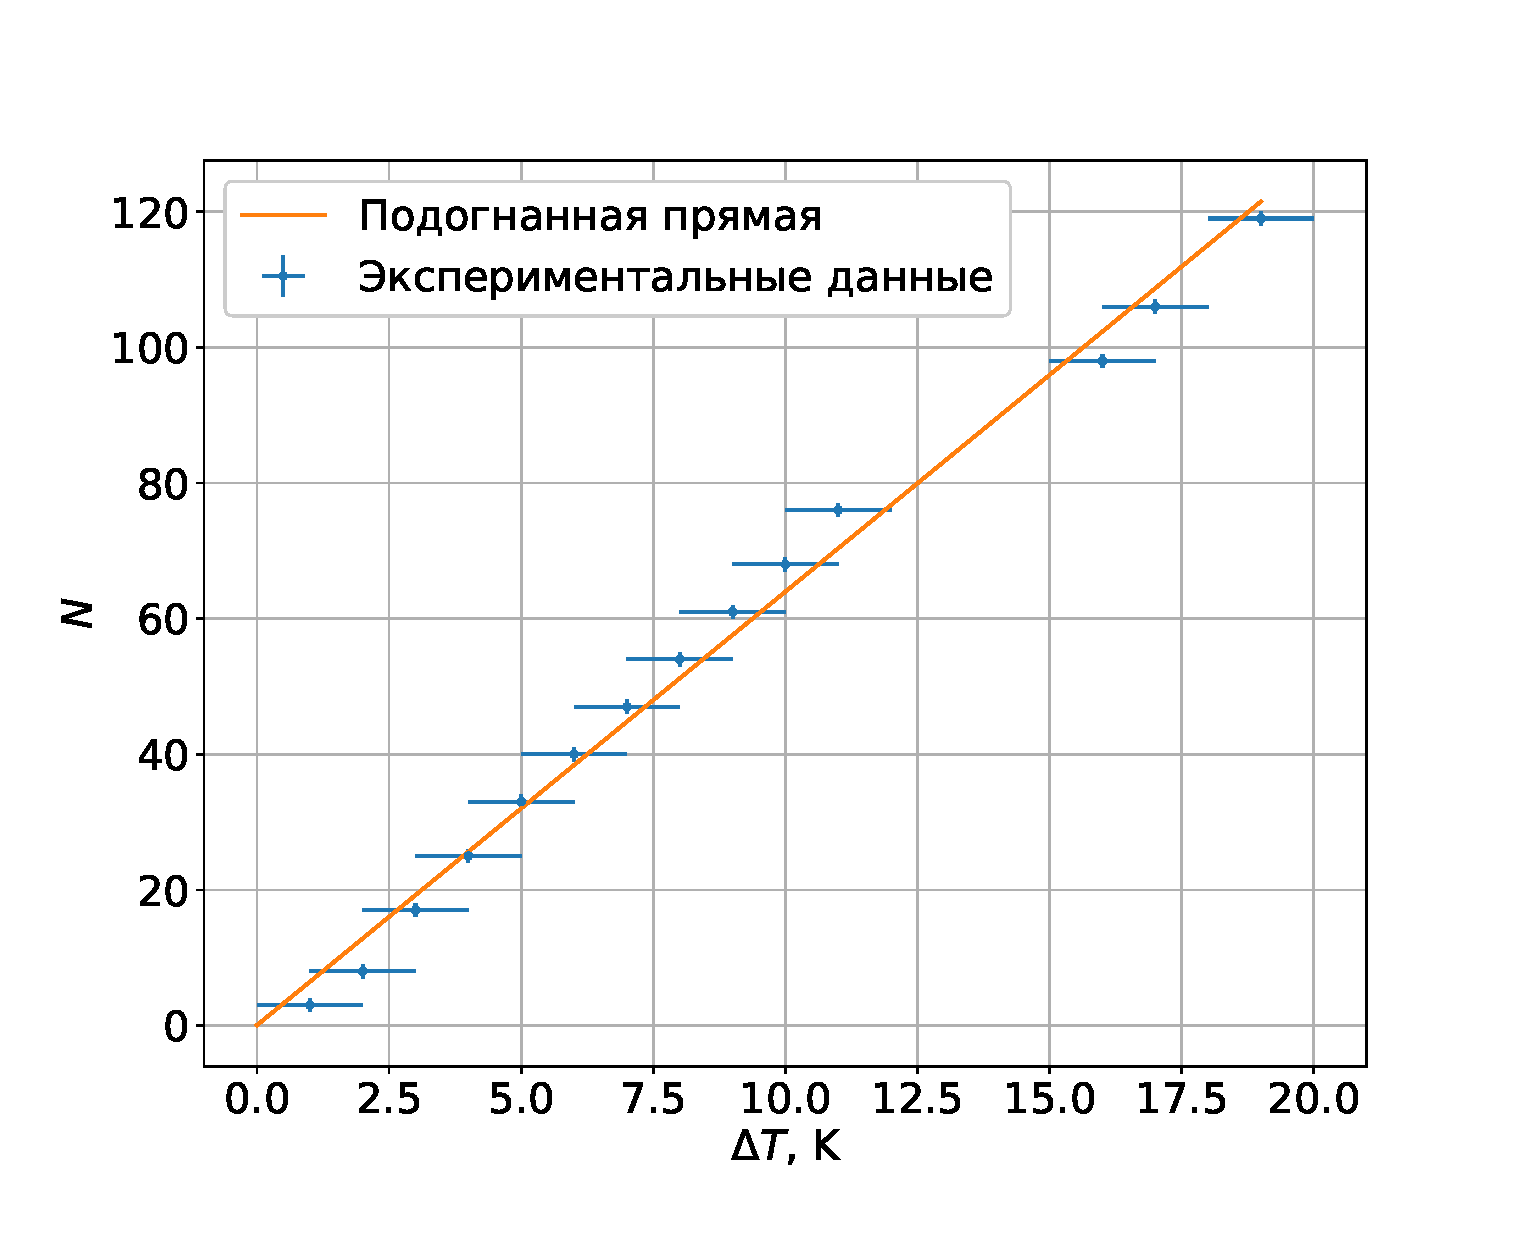
\includegraphics[width=1\linewidth]{exp13.eps}
\caption{\label{fig:epsart}График зависимости количества переходов от температуры стержня}
\end{figure*}
После подгонки прямой, получаем значение коэффициента теплового расширения $\alpha = 18.6 \pm 1$ $MK^-1$
\section{Выводы}
\begin{itemize}
    \item Изучены принципы работы интерферометра Майкельсона
    \item Найдены коэффициенты преломления нескольких пластинок из орг-стекла: $n_{\text{тонкая}} = 1.59 \pm 0.03, n_{\text{толстая}} = 1.43 \pm 0.05$
    \item Найдена спектральная ширина лазера $\Delta \lambda \approx 0.15$ нм
    \item Найден коэффициент теплового коэффициента расширения стали $\alpha = 18.6 \pm 1$ $MK^-1$
\end{itemize}
\nocite{*}

\bibliography{apssamp}

\end{document}
